% !TEX root = ../main.tex

\chapter{Methodology}
\label{chapter:Methodology}
We identify two main challenges with the single observation sparse reward setup. \\
\section{Curse of Dimensionality}
\label{COD_AC}
As introduces in \ref{COD}, the evidence for a model scales approximately inversly proportinal to the exponent of the dimension on which it acts. In MDPs, the 
actor $\pi$ acts on the observation space and returns an action from the action space. A probabalistic actor defines a probability distribution on the set 
of actions $\mathcal{A} \in \mathcal{R}^m$ and observations $\mathcal{O} \in \mathcal{R}^n$ as $\pi(a|o) = \frac{p(a,o)}{p(o)}$. 
Thus the dimension on which the actor acts on, is $n \times m$ with $\pi:\mathcal{R}^m \times \mathcal{R}^n \rightarrow \mathcal{R}$.\\
Similarely, the critic $Q$ usually defines a function on $\mathcal{A}$ and $\mathcal{O}$ to the comulative discounted expected value 
$Q:\mathcal{R}^m \times \mathcal{R}^n \rightarrow \mathcal{R}$, while TQC defines the critic as a quantile distribution: 
$Q:\mathcal{R}^m \times \mathcal{R}^n \rightarrow \mathcal{R}^k$ with $k$ quantiles.\\
We have shown in \ref{POMDP}, that in a POMDP, the observation space grows linear in time. Together with the result from \ref{COD} we conclude, that we have 
exponentially less evidence with sequence length $T$ for our model in the POMDP setting.\\
To counter this problem, we want to get rid of the time dependency of the belief state. To do this, 
we make the observation, that our case with the single observation at the beginning is a special case of a POMDP. Usually, 
we need to know all previous obervsations, as they can give us additional information about the believe state. However, as we don't have subsequent information 
after the initial observation, the only knowledge we have to include to calculate our believe state are the actions, that the policy took. As introduced in \ref{pomdp_bayes}, the optimal believe state 
update in the general POMDP case using bayes theorem is given by:
\begin{equation}
    b_{t+1}(s') = \frac{\mathcal{Z}(s', o_{t+1}) \sum_{s \in \mathcal{S}} \mathcal{T}(s, a_t, s') b_t(s)}{\sum_{s'' \in \mathcal{S}} \mathcal{Z}(a_t, s'', o_{t+1}) \sum_{s \in \mathcal{S}} \mathcal{T}(s, a_t, s') b_t(s)}
\end{equation}
. In our case, we can rewrite this as:
\begin{equation}
    b_{t+1}(s') = \frac{\mathcal{Z}(s', o_{0}) \sum_{s \in \mathcal{S}} \mathcal{T}(s, a_t, s') b_t(s)}{\sum_{s'' \in \mathcal{S}} \mathcal{Z}(s'', o_{0}) \sum_{s \in \mathcal{S}} \mathcal{T}(s, a_t, s') b_t(s)}
\end{equation}
. $\mathcal{Z}(s'', o_{0})$ is constant for $t>0$, so we get:
\begin{equation}
    b_{t+1}(s') \propto \sum_{s \in \mathcal{S}} \mathcal{T}(s, a_t, s') b_t(s) \quad | t > 0
\end{equation}
\begin{equation*}
    b_{0}(s') \propto \mathcal{Z}(s', o_{0})
\end{equation*}
. If we assume a deterministic policy $\pi(a|b) \rightarrow a_{\pi}(b)$, the update step can be written as:
\begin{equation}
    b_{t+1}(s') \propto \sum_{s \in \mathcal{S}} \mathcal{T}(s, a_{\pi}(b_t), s') b_t(s)
\end{equation}
. By using this update step recursively until we get to $b_{0}$, we see, that the believe state at time $t$ only depends on the initial observation $o_0$
the transition probability $\mathcal{T}$ and the number of recursion steps $t$. Using this insight, we can rewrite the belief state at timestep $t$ like:
\begin{equation}
    b_{t+1}(s') \propto \mathcal{Z}(s_0, o_{0}) \mathcal{T}(s_0, s', t)_{\pi}
\end{equation}
, where $\mathcal{T}(s_0, s', t)_{\pi}$ indicates that the normalized transition function depends on the timestep $t$ and policy $\pi$.\\
With this formulation, we can rewrite the policy 

\begin{equation}
    \pi(a|b) : \mathcal{R}^m \times \mathcal{R}^{n T} = \pi(a|o_0, t): \mathcal{R}^m \times \mathcal{R}^{n} \times 1.
\end{equation}
We call this a strong inductive belief state bias for the single observatino POMDP, as it forces the assumption of a deterministic and constant policy $\pi$. 
In our method, we implement a weak inductive bias, which is motivated by this observation: We use transformer encoder type architecture, which inputs are 
the repeated initial observation plus a positional encoding. We then use a single pass through the network, which means it does not work autoregressively and 
relies less on former actions to determin action at time point $t$. We test this hypothesis by using baselines that have the strong inductive bias, as well as 
using the transformer in autoregressive mode. \\

\section{Update Error}
As we only have a single observation, our model has to learn the dynamics of the MDP in order to predict the reward signal at time point $t > 1$. In \cite{NEURIPS2020_b5c01503} 
it has been shown, that learning a transition model for an mdp has a quadratic error bound in $\gamma$ thus we expect quadratic error with the length of the horizon. 
However, we identify that this challange also grants us a unique improvement over previous actor critic methods. By predicting whole sequences of actions at once, 
we show that we can eliminate errors in the update step of the actor and critic.\\
All parametrized actor critic mehtods are technically speaking off policy, as the critic value is bootstrapped with former estimates. Once the actor is updated, the 
critic target moved, on which the actor was updated. Intuitively, when the policy is changed to choose a different action at time point $t$, it might also change 
the policy to choose different actions at 
all subsequent time points, which changes the value function. This leads to unstable update behaviour and is the main reason, why algorithms like PPO try to 
make sure, that changes to the policy are limited. This update instability is specifically challenging in our one observation environment, as the policy does not 
get updates of the state of the environment it is currently in. \\
Formally, let's define the objective function $J(\phi, \theta(\phi)) = \mathbb{E}_{\tau \propto \pi(\phi)}\left[Q_{\theta(\phi)}\right]$ for actor critic methods as the function we whish to optimize to learn the optimal policy. 
$Q_{\theta(\phi_i)}$ indicates the $Q$ function for policy $\pi_{\phi_{i}}$ parametrized by parameters 
$\theta(\phi_i)$. For example, DDPGs policy update rule \ref{AC_general_update} is written as:
\begin{equation}
    \nabla_{\phi} J(\phi, Q(\theta(\phi))) = \mathbb{E}_{\tau \sim p(\tau | \pi_{\phi})} \left[\nabla_{\phi} \log \pi(a_t|s_t;\phi) Q_{\theta, \pi_\phi}(a_t, s_t) \right].
\end{equation}
. Note that generally, we do not have access to $\theta(\phi)$, but only an approximation given the limited data we have collected. Let us denote the actual 
$Q$ function we have as $Q(\theta(\phi) + \epsilon)$, where $\epsilon$ indicates an error between the optimal parameters and the actual parameters.
Let us now for simplicity assume, that $\phi$ and $\theta$ are one dimensional. A generalisation to n dimensions is straight forward, but less readable. We want 
to estimate the update error to $\pi$ from the objective $J$. The proper derivative is given by:
\begin{equation}
    \nabla_{\phi} J(\phi, \theta(\phi)) = \frac{J(\phi + \delta \phi, \theta(\phi + \delta \phi)) - J(\phi, \theta(\phi))}{\delta \phi} + \mathcal{O}(\delta)
\end{equation}
with 
\begin{equation}
    J(\phi + \delta \phi, \theta(\phi + \delta \phi)) = J(\phi, \theta(\phi)) + \left[ 
        \frac{\partial J}{\partial \phi} + \frac{\partial J}{\partial \theta} \frac{\partial \theta}{\partial \phi}
    \right] \delta \phi  + \mathcal{O}(\delta^2)
\end{equation}
, where we used the chain rule and taylor's theorem. 
We can express this in terms of the parametrs $\theta(\phi) + \epsilon$:
\begin{equation}
    \nabla_{\phi} J(\phi, \theta(\phi)) = \nabla_{\phi} J(\phi, \theta(\phi) + \epsilon) - \nabla_{\phi} J(\phi, \theta(\phi)) + \nabla_{\phi} J(\phi, \theta(\phi))
\end{equation}
\begin{equation*}
    = \nabla_{\phi} J(\phi, \theta(\phi)) + \epsilon_{\nabla_{\theta}}
\end{equation*}
. Note that $\nabla_{\phi} J(\phi, \theta(\phi) + \epsilon)$ is not a properly defined derivative. To rigorously capture the stochastic dependence of $\theta(\phi)$ 
given a dataset $\mathcal{D}^n$ with $n$ transitions, 
we could formulate $\theta(\phi)|\mathcal{D}_n$ as n boundary conditions. Together with a suitable regularizor, we can then find $\theta_{\epsilon, n}(\phi)$. We omit 
this step, as we are only interested in the fact that there is an error, not the exact value of it.\\
In actor critic policy updates, $\theta$ is assumed a constant, thus the actor derivative 
$\widetilde{\nabla}_\phi J$ of $J$ is given by:
\begin{equation}
    \widetilde{\nabla}_\phi J(\phi, \theta) =  \frac{J(\phi + \delta \phi, \theta) - J(\phi, \theta)}{\delta \phi} + \mathcal{O}(\delta)
\end{equation}
. 
Again using $\theta(\phi) + \epsilon$ we get:
\begin{equation}
    \widetilde{\nabla}_\phi J(\phi, \theta + \epsilon) = \widetilde{\nabla}_\phi J(\phi, \theta) + \epsilon_{\widetilde{\nabla}_{\theta}}
\end{equation}
We can now derive the update error in the actor update:
\begin{equation}
    \label{equation:general_update_error}
    \nabla_{\phi} J(\phi, \theta(\phi)) - \widetilde{\nabla}_\phi J(\phi, \theta) = \nabla_{\phi} J(\phi, \theta(\phi) + \epsilon) - \epsilon_{\nabla_{\theta}} - \widetilde{\nabla}_\phi J(\phi, \theta(\phi) + \epsilon) + \epsilon_{\widetilde{\nabla}_{\theta}}
\end{equation}
\begin{equation*}
    = \epsilon_{\widetilde{\nabla}_{\theta}} - \epsilon_{\nabla_{\theta}} + \frac{\partial J}{\partial \theta} \frac{\partial \theta}{\partial \phi}
\end{equation*}
. We will call $\epsilon_{\widetilde{\nabla}_{\theta}} - \epsilon_{\nabla_{\theta}}$ the  \textbf{function approximator error}. \\
Recall that $J(\phi, \theta(\phi)) = \mathbb{E}_{\tau \propto \pi(\phi)}\left[Q_{\theta(\phi)}\right]$, so the partial derivative $\frac{\partial J}{\partial \theta} = 1$, 
as the expectation commutes with the derivative. This leaves us with estimating $\delta \frac{\partial \theta}{\partial \phi}$. Again using taylor's theorem, we get 
\begin{equation}
    \label{dist_shift_error}
    \delta \frac{\partial \theta}{\partial \phi} = \theta(\phi + \delta) - \theta(\phi) + \mathcal{O}(\delta).
\end{equation}
We will call this error the \textbf{distribution shift error}.\\
While this derivation assumes direct policy gradient to update the actor, other actor critic policy update methods like the minimisation of a KL divergence as 
proposed is SAC will have similar terms (\cite{SAC}, equation 13).

\subsection{Distribution Shift Error}
\label{dist_shift_error}
From \ref{dist_shift_error} we see, that the error of the update of $\pi$ is proportinal to the change in the 
expected value $J(\pi)$.\\ 


In our aproach, we want to decouple the critic from the actor to set the distribution shift error to zero. To do so, let's see where the difference between 
$\theta(\phi)$ and $\theta(\phi + \delta)$ comes from. Recall when we write $\theta(\phi)$ we mean $Q_{\theta}(a,s|\pi_{\phi})$:
\begin{equation*}
    Q_{\theta}(a,s|\pi_{\phi}) = \mathbb{E}_{(a_t \propto \pi_{\phi}(s_t), s_t \propto T(s_{t-1}, a_{t-1}, s_t))|a_0=a, s_0=s}\left[\sum_t \gamma^t r(a_t, s_t)\right]
\end{equation*}
from that we get
\begin{equation}
    Q_{\theta }(a,s|\pi_{\phi + \delta}) - Q_{\theta}(a,s|\pi_{\phi}) != 0 
\end{equation}
\begin{equation*}
    \text{ if } \pi_{\phi + \delta}(a|s) != \pi_{\phi}(a|s)
\end{equation*}
except for degenerate cases. We propose a whole sequence actor critic, where, given an observation, the actor proposes the whole sequence of actions it will 
take and the critic uses the whole sequence of actions to predict all immediate rewards. The new $C_{\text{whole sequence}}$ is thus defined on an observation $o$ and a 
sequence of actions: 
\begin{equation}
    (a_{1,...,T}) \propto \pi_{\text{whole sequence}}(a_{1,...,T}|o)
\end{equation}
\begin{equation*}
    c_{\text{whole sequence}}(t, o, a_{1,...,T}) = \mathbb{E}_{s_t \propto \tau_t}\left[r(a_t, s_t)\right]
\end{equation*}
, where $\tau_t$ indicates the trajectory until timestep $t$ and $c_{\text{whole sequence}}(t, o, a_1, ..., a_T)$ is the expected reward at time step $t$. \\
Note, that as there is no dependency of $C$ on $\pi$, the distribution shift error \ref{dist_shift_error} is zero. The downside of this approach is, that the 
critic has to predict the MDP, to predict the correct reward after the action sequence $a_{1, ... t}$. While predicting an MDP entailes a quadratic error in 
the sequence lenght as shown in \cite{NEURIPS2020_b5c01503}, it has been shown to be useful for example as a regularizor in \ref{GAIL_POMDP} and as a proxy 
loss in \ref{MUESLI}. Note, that our formulation does not train the policy to predict the exact observations at time step t, but rather it is trained to 
only predict the expected reward. 
In our discussion of \ref{GAIL_POMDPS} we stated, that predicting exact observations is unnecessarly hard and not optimally aligned with the actual objective. 
Our whole sequence critic only has to learn a value equvialent MDP \ref{https://arxiv.org/abs/2011.03506}.\\
While our approach is generally applicable in all MDPs, it is specifically usefull in our environment with only one observation, as in this setup, we can't do 
better then to predict all actions and the reward $T$ steps into the future, as we don't get any other signal.\\ \\

\subsection{Function Approximation Error}
\label{func_app_error}
Recall the function approximator error $\epsilon_{\widetilde{\nabla}_{\theta}} - \epsilon_{\nabla_{\theta}}$ in \ref{equation:general_update_error} was derived from the observation, that our $\theta(\phi)$ is underdetermined 
given limited data $\mathcal{D}^n$. \\
Intuitively, even if the distribution shift error was zero, meaning we knew perfectly the value 
$C((t, o, a_{1,...,T}) \in \mathcal{D}^n)$ of a given action sequence, we don't know the value of an arbitrary action sequence \\
$C((t, o, a_{1,...,T}), o \in \mathcal{D}^n, a_{1,...,T} \notin \mathcal{D}^n)$.\\
To mitigate this error, we want to decouple the actor update from the critic by rephrasing the actor update as an imitation learning problem. 
Let's say we have $m$ expert demonstrations in our dataset. 
Like in imitation learning, we define the update step to our actor as
\begin{equation}
    \Delta \phi = \nabla_{\phi} \mathbb{E}_{(o, a_{t}) \in \mathcal{D}_E, t \in \{1, ..., T\}}\left(\sum_n \pi_{\phi}(o)_{t, n} - a_{t, n}\right)^2
\end{equation}
, where we use a whole sequence actor 
$\pi(o):\mathcal{R}^m \rightarrow \mathcal{R}^{n \times T}$ with an $n$ dimensional action space and $T$ timesteps per trajectory. The index $t$ denotes the $t$th action of the sequence and the index $n$ denotes the $n$th dimension of 
the action. For probabalistic policies, we can use the update rule as stated in \ref{prob_imitation_learning}.\\
This leaves us with the question of how to improve our policy beyond what it can learn from the initial set of expert trajectories. To do this, we propose to use 
the critic in inference time. Let $a_{\pi}(o)$ be the actions proposed by the actor and $c(a_{\pi}(o), o)$ be the immediate predicted rewards by the critic. 
We can now find the gradient of the critic values $c$ by the actions to define new actions: $a_{i+1} = a_i + \nabla_{a}c(a, o)$, as the predicted rewards are a 
function of the actions. This step is repeated k times, to find new actions using the critic in inference time. This usage of the critic in inference time 
is the reason, why we call this method "active critic". To be more precise, in our setup we use the critic to predict only the reward of the last state, as we are 
in the sparse reward setting. A generalisation to dense rewards is straight forward. Moreover, we don't use gradient ascent, as it can be unstable, because with 
higher predicted values, the gradient also increases. Instead, we use gradient descent on $J_{c, a, o} = (c(a, 0) - 1)^2$. This is a natural choice, as we can 
choose reward 1 for the success cases and reward 0 for the failure cases. In this sence, we aim to optimize the predicted probability, that actions $a$ will lead 
to a success, given observations $o$. An overview of the algorithm can be seen in figure {AC algo}. The new trajectory $a_{c, o}$ found by unsing the critic, will 
be added to the set of trajectories for the critic and to the set of expert trajectories, if it was a success. \\
With this setup, our algorithm is truly on policy, while beeing able to use all data collected from expert demonstrations and during training time. The actor is 
model free, while the critic is weakly grounded model based, as it learns to predict the dynamics of the MDP. In this sense, it is close to MuZero and MuEsli, 
but our architecture enables search on continuous action space, which is not possible in MuZero and MuEsli. 
"Monte-Carlo Tree Search in Continuous Action Spaces with Value Gradients" does search on continues action space, but requires the knowledge of the transition model. 
To the authors knowledge, active critic is the only search based algorithm on a continuous action space with no prior access to the transition model.

\subsection{Average Actions Problem}
\label{avr_action_problem}
So far, we have assumed that the trajectories in the dataset of the actor are sampled from an expert. This implies deterministic actions, given an observation. 
In our algorithm, most trajectories in the actor dataset are the result of the search for suitable actions given the current critic. This means we could find
multiple trajectories for the same observation, given that usually multiple action sequences will successfully solve a problem. The actor is trained to miminize 
the $L_2$ distance to all trajectories with the same input $o$, as defined in \ref{actor_objective}. It is not guaranteed and in fact unlikely, that the 
average trajectory will also solve the problem. To illustrate this point, let's say our objective 
is to navigate from point A to point B around an obstacle C. Assume we found two successful trajectories 
$a_1$ and $a_2$ for observation $o$, which encodes the position of A, B and C. Given our algorithm, both trajectories are added to the actor dataset. 
The actor is now trained to minimze the $L_2$ distance, thus it will output the average of $a_1$ and $a_2$ given $o$, which might be a straight line from A to B 
through C and thus not a successful trajectory. \\
To prevent this problem, we whish to disambiguate the actions $a_1$ and $a_2$. We propose an additional network we call the planner $P$. $P$ takes as an input 
the action sequence $a$ and outputs a low dimensional encoding we call the plan $p_a$ of the sequence $a$: 
$P:\mathcal{R}^{T\times n} \rightarrow \mathcal{R}^{d_p},\ p(a) = p_a$, with action dimension $n$, sequence length $T$ and plan dimension $d_p$. This encoding is then fed into the actor together 
with the observation $o$: $a = \pi(o, p_a)$. Now the actor can learn both trajectories disjunctly. However, during inference time, we don't have access to an action sequence 
that would solve the problem to give to the planner $P$. Instead, we define the output of the planner for all action sequences that were initially provided as 
expert trajectories as the zero vector. We can do this, as long as the expert, from which the initial trajectories were sampled, is deterministic, or we make sure 
no two same observations are part of the initial expert trajectories. In inference time, we can then set the plan to the zero vector. 

\subsection{Inference Time Search}
In the derivation of the AC algorithm, we have used the gradient signal from the critic on the actions. As our approach is completely parametrized, we can calculate 
the gradient with respect to the actor, the planner, and also the observation and the plan. In "Noether Networks: Meta-Learning Useful Conserved Quantities" \cite{https://arxiv.org/abs/2112.03321}, 
the authors aim to reconstruct a video sequence 
using conserved properties of the underlying physics. While a different problem setup, they also have a high dimensional derivative with respect to a 
generated output. The authors find, that 
building the gradient with respect to the generator and then regenerating the output performs better, then directly optimizing the output. They hypothesize this 
may be, because the generator has some knowledge about the action space. Following this insight, we found that updating the weights of the actor with respect to the 
critic gradient works best. This update rule can be written as:
\begin{equation}
    a_{i+1} = \pi_{\theta_{i+1}}(o, p(a_i))
\end{equation}
\begin{equation}
    \theta_{i+1} = \theta_i - \alpha_{inf} \nabla_{\theta} (C(\pi_{\theta}(o, p(a_i)), o) - 1)^2
\end{equation}
, where we used the planner network to compute $p(a_i)$ and $p(a_0) = 0$ for the first input to the actor network. 
We do not apply the updated weights to the actor after the inference, but only use them in inference time for the given trajectory. 

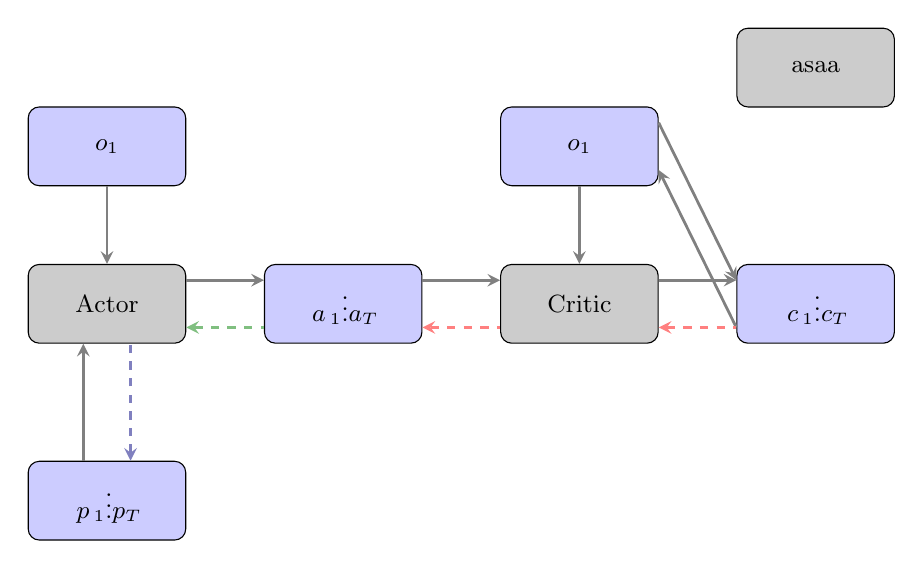
\begin{tikzpicture}[>=stealth,font=\small]
    
    % Define node styles
    \tikzstyle{observation_block_1} = [draw, rounded corners, fill=blue!20, minimum width=2cm, minimum height=1cm, text centered]
    \tikzstyle{actor_block} = [draw, rounded corners, fill=black!20, minimum width=2cm, minimum height=1cm, text centered]
    \tikzstyle{critic_block} = [draw, rounded corners, fill=black!20, minimum width=2cm, minimum height=1cm, text centered]
    \tikzstyle{actions_block} = [draw, rounded corners, fill=blue!20, minimum width=2cm, minimum height=1cm, text centered]
    \tikzstyle{critic_reward_block} = [draw, rounded corners, fill=blue!20, minimum width=2cm, minimum height=1cm, text centered]
    \tikzstyle{observation_block_2} = [draw, rounded corners, fill=blue!20, minimum width=2cm, minimum height=1cm, text centered]
    \tikzstyle{plan_block} = [draw, rounded corners, fill=blue!20, minimum width=2cm, minimum height=1cm, text centered]
    \tikzstyle{asd} = [draw, rounded corners, fill=black!20, minimum width=2cm, minimum height=1cm, text centered]
    
    % Draw nodes
    \node [actor_block] (actor) {Actor};
    \node [observation_block_1, above of=actor, yshift=1cm] (observations_vector_1) {$o_1$};
    \node [plan_block, below of=actor, yshift=-1.5cm] (plans_vector) {$\begin{matrix}p_1\\ \vdots\\ p_T\end{matrix}$};
    \node [actions_block, right of=actor, xshift=2cm] (actions_vector) {$\begin{matrix}a_1\\ \vdots\\ a_T\end{matrix}$};
    \node [critic_block, right of=actions_vector, xshift=2cm] (critic) {Critic};
    \node [observation_block_2, above of=critic, yshift=1cm] (observations_vector_2) {$o_1$};

    \node [critic_reward_block, right of=critic, xshift=2cm] (critic_reward_vector) {$\begin{matrix}c_1\\ \vdots\\ c_T\end{matrix}$};
    \node [asd, above of=critic_reward_vector, yshift=2cm] (vvv) {asaa};

    % Draw arrows
    \draw [->, black!50, line width=1pt] (observations_vector_2.east) ++(0, +0.3cm) --node[midway, above] {} (vvv.west |- 0,+0.3cm);
    \draw [<-, black!50, line width=1pt] (observations_vector_2.east) ++(0, -0.3cm) --node[midway, above] {} (vvv.west |- 0,-0.3cm);

    \draw [->, black!50, line width=1pt] (actor.east) ++(0, +0.3cm) --node[midway, above] {} (actions_vector.west |- 0,+0.3cm);
    \draw [<-, green!50!black!50, line width=1pt, dashed] (actor.east) ++(0, -0.3cm) --node[midway, above] {} (actions_vector.west |- 0,-0.3cm);

    \draw [<-, blue!50!black!50, line width=1pt, dashed] (plans_vector.north) ++(+0.3cm, 0) --node[midway, above] {} (actor.south -| 0.3cm,0);
    \draw [->, black!50, line width=1pt] (plans_vector.north) ++(-0.3cm, 0) --node[midway, above] {} (actor.south -| -0.3cm,0);

    \draw [->, black!50, line width=1pt] (observations_vector_1)  --node[midway, above] {} (actor);
    \draw [->, black!50, line width=1pt] (observations_vector_2)  --node[midway, above] {} (critic);



    \draw [->, black!50, line width=1pt] (actions_vector.east) ++(0, +0.3cm) --node[midway, above] {} (critic.west |- 0,+0.3cm);
    \draw [<-, red!50, line width=1pt, dashed] (actions_vector.east) ++(0, -0.3cm) --node[midway, above] {} (critic.west |- 0,-0.3cm);



    \draw [->, black!50, line width=1pt] (critic.east) ++(0, +0.3cm) --node[midway, above] {} (critic_reward_vector.west |- 0,+0.3cm);
    \draw [<-, red!50, line width=1pt, dashed] (critic.east) ++(0, -0.3cm) --node[midway, above] {} (critic_reward_vector.west |- 0,-0.3cm);

\end{tikzpicture}


\section{Algorithm}
The inference of the actor critic algorithm is depicted in algrothm \ref{AC_Inference}.
Following the insights from \ref{COD_AC}, we first repeat the input observation $o_1$ $T$ times and append a positional encoding $p_i$:
\begin{equation*}
    \tilde{o}_{1, ..., T} = [o_1]^T \oplus [p_i]_{i=1}^T
\end{equation*}
. We then generate the plan encoding as a zero vector with $p_a = 0^{T \times d_p}$ with plan dimension $d_p$. The plan and the repeated observation is the input 
of the actor $\pi$:
\begin{equation}
    a^0 = a_{\pi, 1,...,T} = \pi(\tilde{o}_{1, ..., T})
\end{equation}
. The initial action sequence $a^0$ is then optimized given the critic. For example, if we optimize the actions directly, we get:
\begin{equation*}
    a_{i+1} = a_i + \alpha_{inf}\nabla_{a} (c(o_0, a_i) - 1)^2
\end{equation*}
. Then, the trajectory is added to the respective data sets:
\begin{equation}
    \mathcal{D}_{\text{critic}} = \mathcal{D}_{\text{critic}} \cup (o_0, a_k, r_k)
\end{equation}
\begin{equation*}
    \mathcal{D}_{\text{expert}} = \mathcal{D}_{\text{expert}} \cup (o_0, a_k, r_k)\quad |\quad r_k = 1
\end{equation*}
. Note that with expert actions and expert dataset, we don't mean action sequences that were computed by 
a specific expert, for example a human, but rather we mean generally an action sequence, which solves an MDP given an observation $o$. The AC learner might add 
addtional successful trajectories to the expert dataset. \\
\begin{algorithm}
    \caption{Active critic inference}
    \label{AC_Inference}
    \begin{algorithmic}
    \Require Given $\mathcal{D}_{\text{critic}}$, $\mathcal{D}_{\text{expert}}$,  
    $C_{\theta}$, $\pi_{\phi}$, $\alpha_{inf}$, $N$\\
    \State $p_a \gets 0^{T \times d_p}$ \hfill\COMMENT{Initialize plan to zero vector} \\
    \State sample $o_1$ from MDP\\
    \State $\tilde{o}_{1, ..., T} \gets [o_1]^T \oplus [p_i]_{i=1}^T$ \hfill\COMMENT{Add positional encoding $p_i$ to repeated observation} \\
    \State $a^0 \gets \pi(\tilde{o}_{1, ..., T}, p_a)$\hfill\COMMENT{Get initial actions $a^0$ according to policy $\pi$} \\
    \For {$i=1$ to $N$}{
        \State Update action $a^i$ using gradient descent:\\
        \State $a^{i} \gets a^{i-1} + \alpha_{inf} \nabla_{a^{i-1}} (c(\tilde{o}, a^{i-1}) - 1)^2$
    }
    \State Execute actions sequence $a^N$\\
    \State Get reward $r$ based on final state $s_t \propto a^N$\\
    \State Add experience to replay buffers:\\
    \State $\mathcal{D}_{\text{critic}} \gets \mathcal{D}_{\text{critic}} \cup (o_1, a^N_{1, ..., T}, r)$\\
    \If {$r = 1$}{\\
        \State $\mathcal{D}_{\text{expert}} \gets \mathcal{D}_{\text{expert}} \cup (o_1, a^N_{1, ..., T}, r)$\\
    }
    return $\mathcal{D}_{\text{expert}}$, $\mathcal{D}_{\text{critic}}$
\end{algorithmic}
\end{algorithm}

Now we want to derive the update step of the wohle sequence actor as motivated in the function approximation error section \ref{func_app_error}, given an observation 
$o$ and an action sequence $a^{\text{E}}_{1, ..., T}$. 
To prevent the average action problem defined in \ref{avr_action_problem}, we first encode the expert action sequence using our planner $p_a_{\zeta} = P_{\zeta}(a^{\text{E}}_{1, ..., T})$. 
We also build the sequence embedded observation sequence $\tilde{o}_{1, ..., T}$ as described above. From those inputs, we can compute the actions:
\begin{equation*}
    a_{\pi, 1,...,T} = \pi(\tilde{o}_{1, ..., T},p_a_{\zeta})
\end{equation*}
. From this we get the objective function of the actor as:
\begin{equation}
    \label{actor_objective}
    J_{\phi, \zeta} = \mathbb{E}_{(o, a_{t}) \in \mathcal{D}_E,\ t \in \{1, ..., T\}}\left(\sum_n \pi_{\phi}(\tilde{o}_{1, ..., T}, p_a_{\zeta})_{t, n} - a_{t, n}\right)^2
\end{equation}
, where the respective gradient steps are:
\begin{equation*}
    \phi_{i+1} = \phi_i - \alpha_{\phi} \nabla_{\phi}J_{\phi, \zeta}
\end{equation*}
\begin{equation*}
    \zeta_{i+1} = \zeta_ - \alpha_{\zeta_} \nabla_{\zeta_}J_{\phi, \zeta}
\end{equation*}
. The pseudocode is depicted in algorithm \ref{Actor_Update_Alg}.
\begin{algorithm}
    \caption{Actor Update}
    \label{Actor_Update_Alg}
    \begin{algorithmic}
    \Require Given expert demonstrations $\mathcal{D}_{\text{expert}}$, actor $\pi_{\phi}$, planner $P_{\zeta}$, 
    learning rate $\alpha_{\phi}$, learning rate $\alpha_{\zeta}$\\
    \State Sample $(a^{\text{E}}_{1, ..., T}, o_1)$ from $\mathcal{D}_{\text{expert}}$\\
    \State $\tilde{o}_{1, ..., T} \gets [o_1]^T \oplus [p_i]_{i=1}^T$ \hfill\COMMENT{repeat observations and append positional encoding} \\
    \State $p_a \gets $
    \begin{cases}
        p_{\zeta}(a^{\text{E}}_{1, ..., T})\ |\ a^{\text{E}} \notin \text{original expert demonstrations}\\
        0^{T \times d_p}, \text{else}
    \end{cases} \hfill\COMMENT{generate plan $p_a$} \\
    \State $a^\pi_{1,...,T} \gets \pi_{\phi}(\tilde{o}_{1, ..., T}, p_a)$ \hfill\COMMENT{generate actions according to $\pi_{\phi}$} \\
    \State $J_{\pi} = \mathcal{L}_2(a^\pi_{1,...,T}, a^{\text{E}}_{1, ..., T})$ \hfill\COMMENT{compute $L_2$ loss from actions} \\
    \State $\phi \gets \phi_{old} - \alpha_{\phi} \nabla_{\phi}J_{\pi}$\\
    $\zeta \gets \zeta{old} - \alpha_{\zeta} \nabla_{\zeta}J_{\pi}$ \hfill\COMMENT{update $\phi$ and $\zeta$ according to gradients} \\
    \State return $\phi$, $\zeta$
\end{algorithmic}
\end{algorithm}
Following the section distribution shift error \ref{dist_shift_error} and using $\tilde{o}_{1, ..., T}$ the objective function of the whole sequence critic is defined as :
\begin{equation}
    J_{\theta} = \mathbb{E}_{(o, a_{1,...,T}, r_{1,...,T}) \in \mathcal{D}_{\text{critic}},\ t \in {1, ..., T}}\left[(c_{\theta}(t, \tilde{o}_{1, ..., T}, a_{1,...,T}) - r_t)^2\right]
\end{equation}
. The gradient step is:
\begin{equation*}
    \theta_{i+1} = \theta_i - \alpha_{\theta} \nabla_{\theta}J_{\theta}
\end{equation*}
with learning rate $\alpha_{\theta}$. The pseudocode is depicted in algorithm \ref{Critic_Update_Alg}.
\begin{algorithm}
    \caption{Critic Update}
    \label{Critic_Update_Alg}
    \begin{algorithmic}
    \Require Given replay buffer $\mathcal{D}_{\text{critic}}$, critic $C_{\theta}$ and learning rate $\alpha_{\theta}$\\
    \State Sample $(a^{\text{E}}_{1, ..., T}, o_1, r)$ from $\mathcal{D}_{\text{critic}}$\\
    \State $\tilde{o}_{1, ..., T} \gets [o_1]^T \oplus [p_i]_{i=1}^T$ \hfill\COMMENT{repeat observations and append positional encoding} \\
    \State $c \gets C_{\theta}(\tilde{o}_{1, ..., T}, a^{\text{E}}_{1, ..., T})$\hfill\COMMENT{compute expected reward $c$} \\
    
    \State $J_{C} = \mathcal{L}_2(c, r)$ \hfill\COMMENT{compute $L_2$ loss from reward $r$} \\
    \State $\theta \gets \theta{old} - \alpha_{\theta} \nabla_{\theta}J_{C}$\\
    \State return $\theta$
\end{algorithmic}
\end{algorithm}
Putting everything together, we can now define the whole learning paradigm of the active critic, depicted in algorithm \ref{AC_Learner}. The number of update 
steps in inference time $N$ can be used to weigh exploration against exploitation. A high number of update steps means the critic can find very different 
trajectories, then the one proposed by the actor. As these trajectores are further from the distribution on which the critic learned, the confidence of the 
critic score will be lower.
\begin{algorithm}
    \caption{Active critic learner}
    \label{AC_Learner}
    \begin{algorithmic}
    \Require Given expert demonstrations $\mathcal{D}_{\text{expert}}$, sequence length $T$, learning rates $\alpha_{inf}$, $\alpha_{\theta}$, 
    $\alpha_{\phi}$ and $\alpha_{\zeta}$, inference steps $N$ and update steps $N_{\text{update}}$\\
    \State Initialize  $\mathcal{D}_{\text{critic}} = \mathcal{D}_{\text{expert}}$, 
    actor $\pi_{\phi}$, planner $P_{\zeta}$, critic $C_{\theta}$\\
    \While {\text{not converged}}
    {
        \For {$i=1$ to $N_{\text{update}}$}
        {
            $\phi_{new}$, $\zeta_{new}$ = Actor Update \hfill\COMMENT{see algorithm \ref{Actor_Update_Alg}}\\
            $\theta_{new}$ = Critic Update \hfill\COMMENT{see algorithm \ref{Critic_Update_Alg}}\\
        }
        \For {$s=1$ to $N_{\text{samples}}$}
        {
           $\mathcal{D}_{\text{expert}}$, $\mathcal{D}_{\text{critic}}$ = Inference Step \hfill\COMMENT{see algorithm \ref{AC_Inference}}\\
        }
    }
    \end{algorithmic}
\end{algorithm}




